\chapter{Estado del Arte}
\label{ch:sota}

Este capítulo tiene como objetivo principal revisar los conceptos clave y el estado del arte que constituyen la base de esta tesis. Para ello, se ha estructurado el capítulo en tres grandes bloques. En primer lugar, se explorarán las redes programables y softwarizadas partiendo de las redes \gls{sdn}, se seguirá con los algoritmos de red y el uso de la \gls{ai} como tecnologías habilitadoras, y por último, se analizarán diversos casos de uso relevantes que ejemplifican la aplicación práctica de estas tecnologías, como son las \gls{sg} y las redes de sensores \gls{iiot}. 

\section{Las redes \glsentryshort{sdn}}
\label{sec:redes_sdn} 

En este primer bloque se revisan las redes \gls{sdn}, que son la base de las redes programables y softwarizadas. Se explorarán sus características, ventajas y desventajas, así como sus paradigmas de modos de control, según se indicó anteriormente. Además, se analizarán los protocolos y así como los aspectos clave de las vertientes de trabajo del modo de control \textit{in-band}, y cómo podemos explorar dicho modo para favorecer la flexibilidad y control en redes densas y heterogéneas.\\
\\
Las redes definidas por software (\gls{sdn}) representan un nuevo paradigma que rompe con las arquitecturas tradicionales de red. Antes de que apareciera el concepto de \gls{sdn}, como se puede apreciar en la Figura~\ref{fig:sdn_paradigma}, las redes tradicionales solían tener un plano de control unificado en los propios dispositivos, llamado generalmente \textit{Control plane}, en el que se definía la lógica que dictaba cómo se debía llevar a cabo el forwarding de los paquetes, y un plano de datos, conocido como \textit{Data plane}, que se implementaba definiendo su datapath, compuesto por varios bloques de procesamiento para reenviar los paquetes. Ambos planos estarían unificados en un sentido lógico, en un mismo dispositivo. Sin embargo, con la aparición del paradigma de las redes \gls{sdn}, como se muestra en la Figura, los nodos tradicionales de la red verían cómo su plano de control sería delegado a una entidad externa llamada controlador, preserbando su capadicar para manejar los paquetes. En contratste con las arquitecturas tradicionales de la red, donde había que ir configurando equipo a equipo, y donde cada uno de ellos iba a desempeñar una función de red, en las redes \gls{sdn}, el controlador permite configurar y supervisar de manera inteligente el comportamiento de la red a través de aplicaciones software, facilitando una programación flexible y dinámica del entorno de red. Por lo que, aunque se sigan llamando ``switches'' o nodos \gls{sdn}, estos se comportarán según las reglas que le instale el controlador, pudiendo gestionar paquetes como un switch, un router, un firewall, etc. 

\begin{figure}[ht!]
\centering
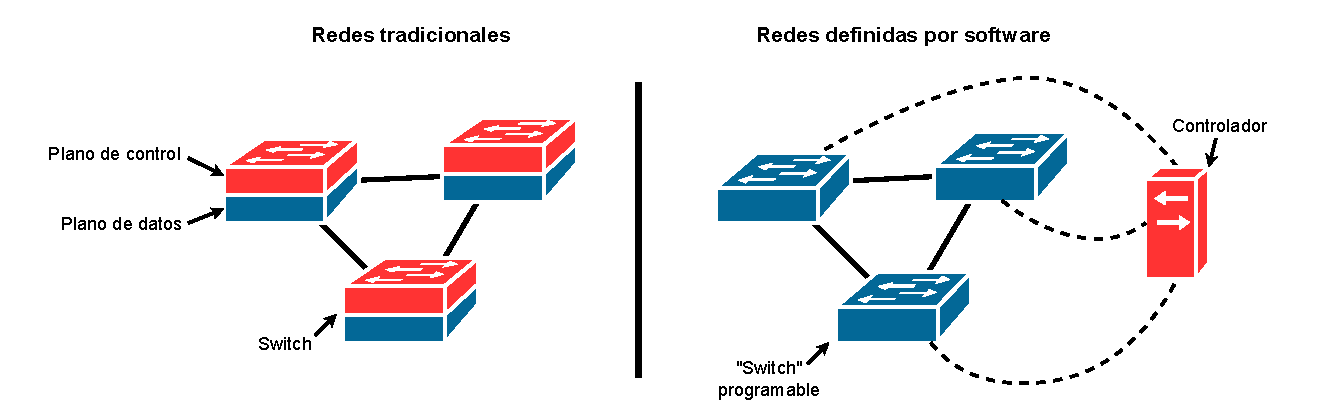
\includegraphics[width=\textwidth]{fig/02_sota/sota_1_sdn_idea.drawio.pdf}
\caption{Paradigma en las redes \glsentryshort{sdn}}
\label{fig:sdn_paradigma}
\end{figure}

La centralización de la gestión simplifica notablemente las tareas del administrador, al proporcionar una visión global del estado de la red y un punto único desde el cual definir su funcionamiento. A través del controlador, las complejas instrucciones de bajo nivel requeridas por los dispositivos de red tradicionales, como switches y routers, las cuales podían variar en función del fabricante, se abstraen mediante interfaces con sintaxis intuitiva, reduciendo la complejidad operativa. Estas capacidades dotan a la red de una gran agilidad y capacidad de adaptación ante cambios o nuevas necesidades, pudiendo conmutar entre distintos perfiles de funcionamiento de forma automática. El simple despliegue de una nueva aplicación sobre el controlador permite modificar de forma coherente el comportamiento de toda la infraestructura, disminuyendo así los costes asociados al mantenimiento, la operación y el despliegue. Además, SDN promueve activamente el uso de soluciones abiertas tanto a nivel de software como de hardware, fomentando ecosistemas interoperables, reduciendo la dependencia de tecnologías propietarias y eliminando barreras de entrada para nuevos actores en el sector.

\subsection{Arquitectura lógica de las redes \glsentryshort{sdn}}
\label{subsec:arquitectura_sdn}

La arquitectura lógica de las redes \gls{sdn} se puede dividir en dos planos, el plano de control y el plano de datos, y además, en tres capas: capa de aplicación, capa de control y capa de infraestructura. En la Figura~\ref{fig:sdn_architecture} se muestra la arquitectura lógica de las redes \gls{sdn}, así como sus interfaces principales de comunicación que más adelante se explicarán.\\
\\
El plano de control, se estructura internamente en dos capas funcionales: la capa de control y la capa de aplicación. Estas se comunican mediante la interfaz norte (northbound interface), que permite a las aplicaciones definir políticas de alto nivel que serán interpretadas y gestionadas por el controlador. Estas capas a menudo se pueden encontrar corriendo en la misma máquina, donde conviven el controlador y las aplicaciones que interactúan con él. Sin embargo, también se puede tener un enfoque distribuido, donde el controlador está en una, máquina, y las aplicaciones en otra, haciendo uso de la interfaz northbound. Por su parte, el plano de datos está conformado por la capa de infraestructura, que engloba los dispositivos físicos de red, principalmente switches \gls{sdn}, responsables del reenvío de paquetes. La interacción entre el plano de control y el plano de datos se realiza a través de la interfaz sur (southbound interface), cuya función es traducir las decisiones del plano de control en instrucciones ejecutables por los dispositivos de red. En este contexto, el controlador actúa como una pieza clave del sistema, asumiendo responsabilidades esenciales como la instalación de reglas de encaminamiento, la monitorización continua del estado de la red y la recopilación de métricas operativas, las cuales serán aprovechadas por todas las aplicaciones que se ejecuten sobre el controlador.

\begin{figure}[ht!]
\centering
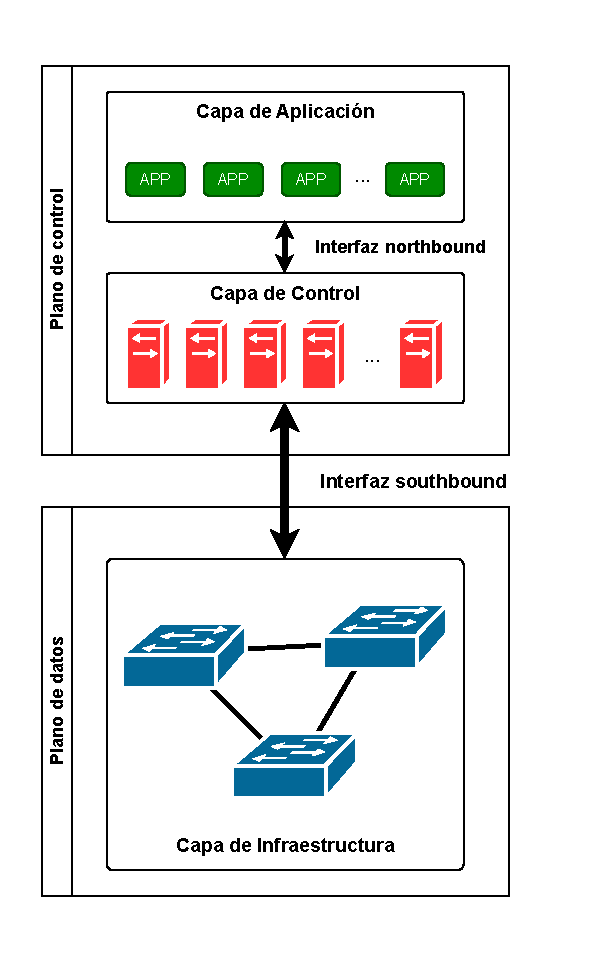
\includegraphics[width=0.5\textwidth]{fig/02_sota/sota_2_sdn_arch_b.drawio.pdf}
\caption{Arquitectura lógica de las redes \glsentryshort{sdn}}
\label{fig:sdn_architecture}
\end{figure}

El plano de datos, por el contrario, no posee lógica de control propia, limitándose a ejecutar las reglas recibidas, como por ejemplo, hacer un reenvío, o descartar paquetes según las reglas establecidas, además de  enviar estadísticas de tráfico al controlador. Esta separación de funciones establece una división clara entre la inteligencia de la red, localizada en el plano de control, y su ejecución, delegada como se ha explicado, al plano de datos. De esta manera, se rompe con el modelo tradicional en el que ambos planos coexistían en un mismo dispositivo de red. Este enfoque modular no solo mejora la escalabilidad y la flexibilidad del sistema, sino que también reduce significativamente los costes de despliegue (\gls{capex}) y operación (\gls{opex}), al concentrar los recursos de cómputo en un nodo centralizado, y simplificar el hardware requerido en los dispositivos de reenvío.\\
\\
Según se ha visto en la Figura~\ref{fig:sdn_architecture}, la arquitectura \gls{sdn} se apoya en una estructura jerárquica formada por tres capas principales: aplicación, control e infraestructura. La capa de aplicación representa el nivel de mayor abstracción dentro del ecosistema \gls{sdn}. Esta capa integra un conjunto de aplicaciones que, apoyándose en los servicios ofrecidos por la capa de control, permiten definir políticas de gestión, \gls{qos}, optimizar el rendimiento de la red y adaptarla dinámicamente a diferentes contextos operativos. Un ejemplo típico de uso es la utilización los servicios de descubrimiento topológico proporcionados por la capa de control, que permiten a las aplicaciones calcular rutas óptimas entre dispositivos de red. Estas aplicaciones suelen desarrollarse empleando lenguajes de alto nivel como Python, Go o C++, con el objetivo de facilitar su portabilidad entre plataformas y maximizar la reutilización del código. No obstante, en la práctica, la existencia de \glspl{api} y entornos de desarrollo específicos para cada plataforma de control, como ONOS, OpenDaylight, Ryu o el nuevo controlador del ecosistema \gls{sdn}, TeraflowSDN, introduce ciertos desafíos en la interoperabilidad y portabilidad del software entre distintas implementaciones. En este sentido, uno de los principales retos actuales de \gls{sdn} sigue siendo la estandarización de interfaces northbound que permitan una integración más fluida y flexible entre aplicaciones y controladores heterogéneos.\\
\\
Descendiendo, la siguiente capa es la capa de control, la cual constituye el núcleo funcional del paradigma \gls{sdn}, albergando la inteligencia centralizada de la red. Actúa como intermediario entre las aplicaciones de alto nivel y los dispositivos físicos de la capa de infraestructura, orquestando tareas críticas como el encaminamiento de flujos, la detección y resolución de fallos, la supervisión continua del estado de la red y la gestión de políticas de seguridad y \gls{qos}. Su papel como middleware se traduce en la capacidad de transformar políticas abstractas generadas en la capa de aplicación en instrucciones simples y concretas que pueden ser entendidas por los nodos \gls{sdn}. Esta capacidad de traducir y escalar la lógica de red permite que un único controlador gobierne cientos o miles de switches de forma eficiente, garantizando escalabilidad y consistencia en entornos distribuidos. Por último, la capa de infraestructura, por su parte, está compuesta por los elementos físicos de la red, fundamentalmente nodos \gls{sdn}, que ejecutan las decisiones tomadas por el plano de control. Estos dispositivos, carentes de lógica propia, cuentan con un agente \gls{sdn} encargado de comunicarse con el controlador a través de la interfaz sur (southbound interface), como por ejemplo, OpenFlow o P4Runtime. Su funcionalidad se reduce al reenvío y descarte de paquetes o la recolección de estadísticas, lo que permite simplificar su diseño y reducir sus requisitos hardware.\\
\\
En cuanto a las interfaces, hay dos, como se ha mencionado anteriormente, la interfaz northbound y la interfaz southbound. La interfaz northbound constituye el canal de comunicación entre la capa de control y la capa de aplicación. Su principal función es ofrecer un punto de acceso lógico al administrador de red, permitiéndole supervisar, configurar y gestionar el comportamiento de la red sin necesidad de interactuar directamente con los mecanismos de bajo nivel que gobiernan los dispositivos físicos. A través de esta interfaz, las aplicaciones pueden programar políticas o solicitudes que serán traducidas por el controlador en instrucciones comprensibles para los elementos de la infraestructura. No obstante, a diferencia de la interfaz southbound, la interfaz northbound carece de una estandarización formal. En consecuencia, la naturaleza y funcionalidad de esta interfaz varían considerablemente en función del controlador \gls{sdn} empleado, cada uno de los cuales suele ofrecer su propia \gls{api} con diferentes modelos de datos, protocolos y lenguajes de interacción.\\
\\
La interfaz southbound constituye el enlace entre la capa de control y la capa de infraestructura dentro de una arquitectura \gls{sdn}. A diferencia de la interfaz northbound, esta sí cuenta con protocolos estandarizados ampliamente adoptados, que permiten la interoperabilidad entre los controladores y los dispositivos de red. Históricamente, el protocolo más representativo ha sido Openflow~\cite{mckeown2008openflow}. En la implementación del protocolo Openflow según se indica en la Figura~\ref{fig:sdn_openflow}, el concepto central es el de flujo (del inglés, \textit{flow}), entendido como un conjunto de paquetes que cumplen determinadas condiciones definidas por el controlador. Estas condiciones se almacenan en las denominadas tablas de flujo (del inglés, \textit{flow tables}), y suelen hacer referencia a valores específicos de campos en la cabecera del paquete o al puerto de entrada por el que se ha recibido.

\begin{figure}[ht!]
\centering
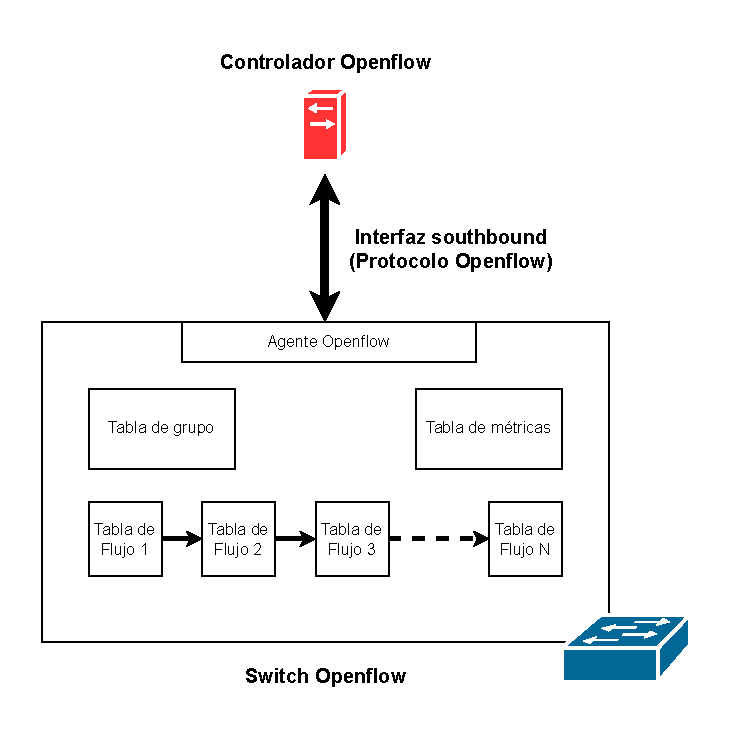
\includegraphics[width=0.7\textwidth]{fig/02_sota/sota_3_sdn_openflow.drawio.pdf}
\caption{Arquitectura básica de switch OpenFlow}
\label{fig:sdn_openflow}
\end{figure}

Cuando un paquete llega a un switch Openflow, empieza a atravesar de forma iterativa las tablas de flujo y cuando este coincide con los criterios de una regla definida en una tabla, se produce una coincidencia (del inglés, \textit{match}), lo que activa un conjunto de instrucciones asociadas a dicha regla. Estas instrucciones pueden incluir el conteo de paquetes, la aplicación de acciones concretas (como reenviar o descartar el paquete), o bien su reenvío hacia otra tabla para un procesamiento adicional. En caso de no darse una coincidencia, se encapsula y se manda al controlador para que este decida que cómo manejarlo. Así, mediante la instalación de estas reglas por parte del controlador \gls{sdn}, se determina el comportamiento de reenvío del switch. La comunicación entre el controlador y los dispositivos se realiza a través de un canal estructurado y seguro, que admite mensajes del controlador al switch, mensajes asíncronos generados por los dispositivos, y mensajes simétricos intercambiables por ambas partes, permitiendo una gestión eficiente y dinámica del estado de red.\\
\\
No obstante, las limitaciones de flexibilidad, extensibilidad y adaptación a nuevas arquitecturas han motivado el surgimiento de alternativas a Openflow. Un ejemplo destacado es el lenguaje \gls{p4}~\cite{bosshart2014p4}, diseñado específicamente para superar las restricciones de OpenFlow. Una de las mayores restricciones que tiene OpenFlow es la especificación de forma explícita de los campos de cabecera sobre los que opera. Estos campos de cabecera han pasado de 12 a 41 campos de cabeceras entre sus versiones 1.0 y 1.5 como se puede ver en la Tabla~\ref{tab:openflow_versions}. Esta evolución ha incrementado la complejidad del protocolo sin proporcionar la flexibilidad necesaria para incorporar nuevas cabeceras o funcionalidades emergentes. 

\begin{table}[ht!]
\centering
\begin{tabular}{|c|c|l|}
\hline
\textbf{Versión} & \textbf{Fecha} & \textbf{Campos de cabecera} \\ \hline
OF 1.0 & Dic. 2009 & 12 campos (Ethernet, TCP/IPv4) \\ \hline
OF 1.1 & Feb. 2011 & 15 campos (MPLS, metadatos entre tablas) \\ \hline
OF 1.2 & Dic. 2011 & 36 campos (ARP, ICMP, IPv6, etc.) \\ \hline
OF 1.3 & Jun. 2012 & 40 campos \\ \hline
OF 1.4 & Oct. 2013 & 41 campos \\ \hline
OF 1.5 & Mar. 2015 & 44 campos \\ \hline
\end{tabular}
\caption{Evolución de versiones del protocolo Openflow y el número de campos de cabecera soportados}    
\label{tab:openflow_versions}
\end{table}

En respuesta a ello, \gls{p4} nació con tres objetivos principales: 

\begin{itemize}
    \item Permitir la reconfiguración del dispositivo en caliente, es decir, cambiar el comportamiento de los switches una vez desplegados.
    
    \item Ofrecer independencia de protocolo, desvinculando el procesamiento de paquetes de protocolos específicos que tengan que estar estandarizados para poder ser gestionados.
    
    \item Proporcionar independencia del hardware, permitiendo que las funcionalidades de procesamiento se definan sin depender de los detalles del dispositivo subyacente. Si bien es cierto que la iniciativa de \gls{p4} nació con este objetivo en mente (\textit{open-hardware}), la realidad es que, en la actualidad, se ha visto como cada fabricante ha implementado equipos que si cumplen con algunas de las arquitecturas de \gls{p4}, pero que cada uno te ofrece unas primitivas de programación diferentes, haciendo que un programa \gls{p4} que corre en un dispositivo de un fabricante no sea totalmente compatible en otro~\cite{hauser2023survey}. 
\end{itemize}

En comparación con Openflow, si nos fijamos en la Figura~\ref{fig:sdn_p4}, podemos apreciar que empleando \gls{p4} se puede definir el cómo el switch va a manejar los paquetes, como los va a procesar y parsear, manteniendo la lógica de las tablas de flujo que teníamos en Openflow, pero ganando en flexibilidad dado que se pueden definir el propio datapath del dispositivo sin depender de un conjunto estandarizado de campos de cabecera. Esto incluso permite que \gls{p4} pueda ser implementado en dispositivos de baja capacidad~\cite{carrascal2020analysis}, al poder ajustar el datapath a la mínima expresión necesaria para cumplir con las necesidades de la red. Al igual que en Openflow se tenía el protocolo de comunicación para la interfaz southbound, \gls{p4} también tiene su propia interfaz de comunicación, llamada P4Runtime~\cite{p4runtime2023}, que permite a los controladores gestionar y programar dispositivos \gls{p4} de forma dinámica. 

\begin{figure}[ht!]
\centering
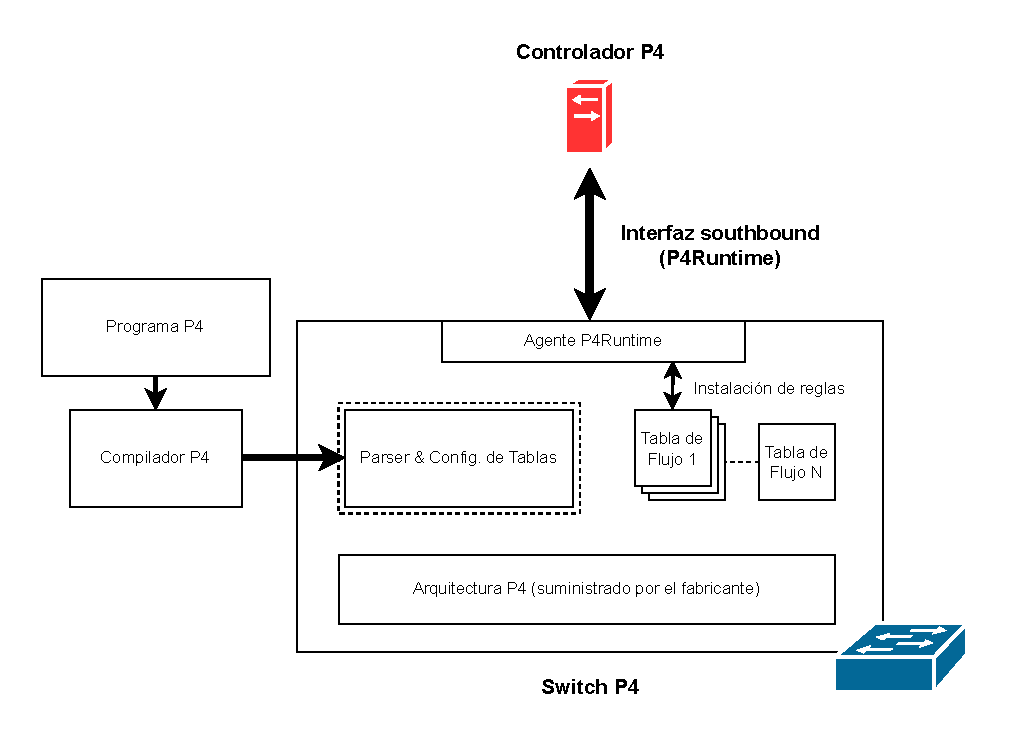
\includegraphics[width=0.9\textwidth]{fig/02_sota/sota_4_sdn_p4.drawio.pdf}
\caption{Arquitectura básica de switch \glsentryshort{p4}}
\label{fig:sdn_p4}
\end{figure}

A diferencia de Openflow, que define un conjunto cerrado de operaciones y estructuras, \gls{p4} y su interfaz P4Runtime introducen la posibilidad de reconfigurar dinámicamente el comportamiento del plano de datos mediante descripciones personalizadas del procesamiento de paquetes. Esto se logra mediante una arquitectura basada en \gls{grpc}, que ofrece cinco tipos de operaciones principales (Write, Read, Set/GetForwardingPipelineConfig y StreamChannel) para gestionar tanto el estado como la lógica interna de los switches programables. De esta forma, \gls{p4} se presenta como una propuesta de evolución de Openflow, orientada a lograr una programabilidad del plano de datos más flexible y escalable, haciendolo ideal para testing y pruebas de concepto de nuevas soluciones de red.\\
\\
Paralelamente, ha ido creciendo otra vía complementaria orientada a la gestión y configuración unificada de dispositivos de red llamada OpenConfig. Esta iniciativa, impulsada mayormente por un consorcio de operadores y fabricantes, propone un conjunto de modelos de datos basados en YANG que permiten describir de forma estandarizada y agnóstica el estado operativo y la configuración de dispositivos de red. A diferencia de OpenFlow o P4Runtime, que se centran en el comportamiento del plano de reenvío, OpenConfig aborda la gestión, configuración, el monitoreo y la automatización de tareas de red a través de protocolos como gNMI o NETCONF. Esto convierte a OpenConfig una herramienta clave para aquellas empresas que buscan una gestión softwarizada y programable de sus infraestructuras ya existentes, dado que permite la integración de dispositivos heterogéneos de diferentes fabricantes bajo un modelo común de gestión. Si bien es cierto que OpenConfig no permite definir explícitamente el plano de datos, a diferencia de Openflow o \gls{p4}, donde se considera que todos los switches o nodos \gls{sdn} equivalen a un único dispositivo lógico gestionado de forma centralizada, OpenConfig propone un enfoque diferente. Esta iniciativa busca establecer un conjunto común de modelos de datos y configuración, independientes del fabricante, para gestionar redes heterogéneas. A diferencia del enfoque \gls{sdn} tradicional, en el que los dispositivos se integran como un único plano de control y datos, los dispositivos gestionados mediante OpenConfig siguen operando como entidades independientes. Ambos enfoques persiguen una mayor transparencia y facilidad de gestión de la red, pero difieren en su grado de abstracción y centralización: mientras \gls{sdn} trata la red como un todo unificado, OpenConfig mantiene la identidad individual de cada dispositivo, facilitando la interoperabilidad en entornos mixtos. Sin embargo, los últimos controladores \gls{sdn} como TeraflowSDN~\cite{teraflowsdn2021}, han comenzado a integrar OpenConfig como una de sus interfaces southboud (además de \gls{p4}), incluso llegando a no implementar Openflow, lo que sugiere una tendencia hacia un nuevo ecosistema de redes \gls{sdn} que combina la flexibilidad de la programación del plano de datos con la estandarización y la gestión eficiente de dispositivos hetereogenos.\\
\\
En este sentido, la evolución de la interfaz southbound no debe entenderse en términos de sustitución de unos protocolos por otros, sino como una diversificación funcional que permite combinar capacidades de reenvío programable, comunicación eficiente y gestión estandarizada según las necesidades específicas de cada red.





\section{Algoritmos de red y \glsentryshort{ai}}
\label{sec:tecnologias_habilitantes}

En este segundo bloque se quieren revisar las principales tecnologías habilitantes que permiten la creeación, control y gestión de las redes programables y softwarizadas. Estas tecnologías son fundamentales para entender el marco de trabajo de la tesis, y cómo, posteriormente, se pueden llegar a aplicar a diferentes casos de uso. 


\section{Casos de uso}  
\label{sec:casos_de_uso}
En este último bloque se revisan los casos de uso más relevantes que se pueden encontrar en la literatura. Estos casos de uso son ejemplos prácticos de cómo las tecnologías habilitantes y las redes programables y softwarizadas se aplican en contextos reales, como las \gls{sg} y las redes de sensores \gls{iiot}. 